\section{Lab: Reti Neurali da zero}
\subsection{Introduzione}

Partiamo dicendo una cosa molto importante: \textbf{per quale motivo usiamo la
    backpropagation?}
\begin{equation}
    \frac{y-b}{x} = w
\end{equation}

Ma possiamo scriverlo come:
\begin{equation}
    (y-b) \cdot x^{-1} = w
\end{equation}

Ora però, se consideriamo:
\begin{itemize}
    \item y il vettore risultante
    \item w la matrice dei pesi
    \item x il vettore di input
\end{itemize}

Calcolare l'inversa di \textbf{x} non è una cosa cosi poco costosa, anzi. Per
questo motivo utilizziamo il training delle reti come la backpropagation e la
discesa del gradiente.

Ora, andiamo più a fondo. Facciamo un esempio più pratico.

\subsection{Esempio pratico}

Immaginiamo di avere un dataset di 2 features e una label da identificate.
%make  atable with x_1 e x_2 and y, with 10 rows
\begin{table}[h!]
    \centering
    \begin{tabular}{|c|c|c|}
        \hline
        $x_1$ & $x_2$ & y \\
        \hline
        1     & 2     & 0 \\
        2     & 3     & 0 \\
        3     & 4     & 0 \\
        4     & 5     & 0 \\
        5     & 6     & 0 \\
        6     & 7     & 1 \\
        7     & 8     & 1 \\
        8     & 9     & 1 \\
        9     & 10    & 1 \\
        10    & 11    & 1 \\
        \hline
    \end{tabular}
    \caption{Dataset di esempio}
    \label{tab:my_label}
\end{table}

Ogni livello di una rete neurale può essere rappresentato attraverso le
\textbf{matrici}.

%fai un grafico di una rete neurale con 2 input, 1 hidden layer da 3 nodi e un output layer da 1 nodo
\begin{figure}[h!]
    \centering
    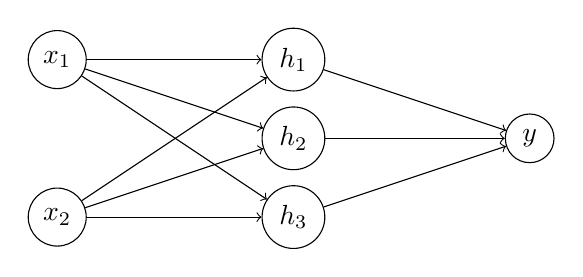
\begin{tikzpicture}
        \node[draw,circle] (x1) at (0,0) {$x_1$};
        \node[draw,circle] (x2) at (0,-2) {$x_2$};
        \node[draw,circle] (h1) at (3,0) {$h_1$};
        \node[draw,circle] (h2) at (3,-1) {$h_2$};
        \node[draw,circle] (h3) at (3,-2) {$h_3$};
        \node[draw,circle] (y) at (6,-1) {$y$};
        \draw[->] (x1) -- (h1);
        \draw[->] (x1) -- (h2);
        \draw[->] (x1) -- (h3);
        \draw[->] (x2) -- (h1);
        \draw[->] (x2) -- (h2);
        \draw[->] (x2) -- (h3);
        \draw[->] (h1) -- (y);
        \draw[->] (h2) -- (y);
        \draw[->] (h3) -- (y);
    \end{tikzpicture}
    \caption{Rete neurale di esempio}
    \label{fig:my_label}
\end{figure}

Ma passiamo alla definizione formale:

\textbf{Definizione Rete Neurale}: Una rete neurale è una tupla:
\begin{equation}
    NN = \{g,l,o,i,fpp\}
\end{equation}
con:
\begin{itemize}
    \item g: il grafico
    \item l: la funzione loss
    \item o: l'ottimizzatore
    \item i: l'inizializzatore
    \item fpp: la fix point procedure
\end{itemize}

\textbf{Nota 1:} l'ottimizzatore intende in quale modo si performa la \textbf{discesa del gradiente.}

\textbf{Nota 2:} l'inizializzatore è la funzione che inizializza i pesi della rete neurale. Ci possono essere diversi algoritmi per gli
inizializzatori, ma non c'è modo di sapere quale funziona meglio, poiché non si può sapere nelle reti neurali.

\subsubsection{Il grafo}

Il solito grafo che abbiamo visto in precedenza è un grafo aciclico diretto. Ha
dei nodi che sono i percettroni, che hanno degli archi composti dai pesi, che
hanno una funzione di attivazione, che prendono in input un valore e ne sputano
fuori uno chiamando la funzione di attivazione sull'input.

\textbf{Nota:} la funzione di attivazione è una funzione non lineare.

\subsubsection{La funnzione loss}

L'obiettivo della funzione loss è quello di misurare la distanza tra il valore
predetto e il valore reale.
\begin{equation}
    L(y,\hat{y}) = \frac{1}{2}(y-\hat{y})^2
\end{equation}

\subsubsection{L'ottimizzatore}

L'ottimizzatore ci permette di trovare una soluzione ottimale \textbf{non
    ottima}, cioé trovare \textbf{il minimo della funzione di loss}. La tecnica che
si usa è quella delle \textbf{discesa del gradiente}.

\subsubsection{Discesa del gradiente}

La discesa del gradiente sfrutta un parametro chiamato \textbf{learning rate}
che permette di capire quanto la discesa del gradiente deve essere veloce. Se
il learning rate è troppo alto, la discesa del gradiente potrebbe non
convergere, se è troppo basso, la discesa del gradiente potrebbe convergere
troppo lentamente.

\textbf{Nota:} il learning rate è un ottimizzatore \textit{molto naive}.

\subsubsection{Inizializzatore}

Il metodo di inizializzazione può cambiare di molto il risultato della rete
neurale. In pratica assegna un valore ai \textit{pesi} e ai \textit{bias}.
Alcuni metodi sono:
\begin{itemize}
    \item Inizializzazione a 0: Questo ha alcuni problemi, perché non si ha
          diversificazione tra i nodi e i nodi nascosti diventano simmetrici.
    \item inizializzazione costante: stessi problemi della precedente
    \item Inizializzazione Random: Si fa seguendo una distribuzione uniforme oppure una
          distribuzione normale.
\end{itemize}

\subsubsection{Fix Point Procedure}

La procedura per il training di una rete neurale è un processo che si basa su
alcuni steps:
\begin{lstlisting}

net CustomNeuralNetwork(...)
initialize_weights_and_biases (net)
optimizer = myOptimizer(...) 
loss_function = myLoss Function(...)
epochs = ... # the number of dataset scans
history = [] # a list containing the loss evolution
for epoch in range(epochs):
    optimizer.reset() # it may have an internal status
    loss = loss_fuction (out_target, net(input)) back_propagation (loss, optimizer, net)
    history.append(loss)
\end{lstlisting}

\subsection{Esempio da zero}
\subsubsection{La funzione Sigmoid}

Spendiamo qualche parola sulla funzione sigmoid, che è una funzione molto
importante per le reti neurali.

In particolare, la funzione avrà un valore di attivazione compreso tra 0 e 1 e,
in particolare, quando l'input è 0, la funzione ha valore 0.5. Se ha un valore
basso, sarà zero e chiaramente se sarà alto avrà valore 1.
\begin{figure}[H]
    \begin{center}
        \begin{tikzpicture}
            \begin{axis}[
                    axis lines = left,
                    xlabel = $x$,
                    ylabel = {$f(x)$},
                ]
                %Below the red parabola is defined
                \addplot [
                    domain=-10:10,
                    samples=100,
                    color=red,
                ]
                {1/(1+exp(-x))};
                \addlegendentry{$\frac{1}{1+e^{-x}}$}
            \end{axis}
        \end{tikzpicture}
    \end{center}
    \caption{Funzione Sigmoid}
\end{figure}

Detto questo, \textbf{per quale motivo è importante?} Se pensiamo
all'\textit{inizializzazione}, che tipi di valori è meglio avere? Avere tutti i
valori a zero porterebbe a valori simmetrici e quindi a problemi di
convergenza. Vogliamo dei valori di pesi che siano \textbf{distribuiti
    uniformemente intorno allo 0.}

\subsection{Tangente Iperbolica TanH}

La funzione TanH è una funzione che ha un valore di attivazione compreso tra -1
e 1 e, in particolare, quando l'input è 0, la funzione ha valore 0. Se ha un
valore basso, sarà -1 e chiaramente se sarà alto avrà valore 1.

\begin{figure}[H]
    \begin{center}
        \begin{tikzpicture}
            \begin{axis}[
                    axis lines = left,
                    xlabel = $x$,
                    ylabel = {$f(x)$},
                ]
                %Below the red parabola is defined
                \addplot [
                    domain=-10:10,
                    samples=100,
                    color=red,
                ]
                {tanh(x)};
                \addlegendentry{$tanh(x)$}
            \end{axis}
        \end{tikzpicture}
    \end{center}
    \caption{Funzione TanH}
\end{figure}

\subsection{ReLu}

La funzione ReLu è una funzione che ha un valore di attivazione pari a 0 quando
l'input è negativo e ha un valore di attivazione pari all'input quando l'input
è positivo.

\textbf{Parole di Adornetto:} E' buona? Si. E' stabile? Si. Perché? Boh.

\begin{figure}[H]
    \begin{center}
        \begin{tikzpicture}
            \begin{axis}[
                    axis lines = left,
                    xlabel = $x$,
                    ylabel = {$f(x)$},
                ]
                %Below the red parabola is defined
                \addplot [
                    domain=-10:10,
                    samples=100,
                    color=red,
                ]
                {max(0,x)};
                \addlegendentry{$max(0,x)$}
            \end{axis}
        \end{tikzpicture}
    \end{center}
    \caption{Funzione ReLu}
\end{figure}

\subsection{Scalare i valori}

Skip molto avanti riguardo l'esempio, ma si parla di scalare i dati.

Lo scaling dei dati è un'operazione importante nel machine learning perché i
dati possono essere su scale diverse e questo può causare problemi durante
l'allenamento del modello. Ad esempio, se abbiamo due variabili di input, una
che varia da 0 a 1 e l'altra che varia da 0 a 1000, la seconda variabile avrà
un impatto molto maggiore sull'output del modello rispetto alla prima. Ciò può
portare a problemi come l'overfitting, in cui il modello si adatta troppo ai
dati di addestramento e non generalizza bene sui dati di test.

Per risolvere questo problema, si utilizzano tecniche di scaling dei dati per
portare tutte le variabili su una scala comune. Ci sono diverse tecniche di
scaling, come la normalizzazione e la standardizzazione, che possono essere
utilizzate a seconda del tipo di dati e del modello utilizzato.

Le funzioni di attivazione, come la funzione ReLU, possono anche essere
influenzate dalla scala dei dati di input. Se i dati non sono scalati
correttamente, la funzione di attivazione potrebbe produrre valori che non
permettono un allenamento corretto del modello. Lo scopo dello scaling dei dati
è quello di mantenere i dati intorno allo 0, in modo che le funzioni di
attivazione possano produrre valori che permettono un allenamento corretto del
modello.

\begin{itemize}
    \item Standardizzazione: La standardizzazione è una tecnica di scaling dei dati che
          assume che i dati siano distribuiti normalmente all'interno di ogni feature e
          li scala in modo che la distribuzione abbia una media uguale a 0 e una
          deviazione standard uguale a 1. Questa tecnica funziona bene quando i dati
          hanno una distribuzione normale, ma non funziona bene se i dati hanno una
          distribuzione non normale.
    \item Normalizzazione: La normalizzazione è una tecnica di scaling dei dati che scala
          i valori di ogni feature in modo che siano compresi tra 0 e 1. Questa tecnica
          funziona bene quando i valori di input non hanno una distribuzione normale. Ad
          esempio, se i valori di input sono compresi tra 0 e 1000, la normalizzazione li
          porterà su una scala compresa tra 0 e 1.
\end{itemize}

\subsection{Plottare la loss}

La funzione loss è una misura dell'errore del modello durante
l'allenamento. L'obiettivo dell'allenamento è quello di minimizzare la funzione
loss, ovvero di ridurre l'errore del modello. Durante l'allenamento, il modello
viene eseguito su un set di dati di addestramento e la funzione loss viene
calcolata per ogni esempio di addestramento. L'errore totale del modello è la
somma di tutte le funzioni loss per ogni esempio di addestramento.

L'allenamento del modello avviene in epoche, ovvero in cicli di esecuzione su
tutti i dati di addestramento. L'obiettivo è che la funzione loss diminuisca ad
ogni epoca, ovvero che l'errore del modello diminuisca man mano che il modello
viene addestrato su più dati. Se la funzione loss non diminuisce ad ogni epoca,
significa che il modello non sta imparando abbastanza dai dati di addestramento
e potrebbe essere necessario modificare l'architettura del modello o i
parametri di addestramento.

Se la funzione di loss arriva a 0, vuol dire che \textbf{siamo in minimo globale}, che non è comune.

%make a plot with x = epochs and y = loss and loss reaches 0 at the end, with a curve that goes down
\begin{figure}[H]
    \begin{center}
        \begin{tikzpicture}
            \begin{axis}[
                    axis lines = left,
                    xlabel = $epochs$,
                    ylabel = {$loss$},
                ]
                %Below the red parabola is defined
                \addplot [
                    domain=0:10,
                    samples=100,
                    color=red,
                ]
                {1/(1+exp(x))};
                \addlegendentry{$loss$}
            \end{axis}
        \end{tikzpicture}
    \end{center}
    \caption{Funzione loss}
\end{figure}


Se invece finiami con un grafico che arriva fino a 0.1 e poi si stabilizza, 
potremmo essere in un \textbf{minimo locale}, oppure semplicemente la topologia della Rete
permette di avere questo risultato come massimo risultato.


\subsection{Importante cosa su Gradient Descent}

Lo usiamo per un motivo particolare:
\begin{quote}
    Più andiamo indietro nei layer della rete, maggiori saranno i termini 
    che abbiamo già calcolato, rendendo i calcoli più efficienti.
\end{quote}
Questo è più semplice rispetto ad invertire una matrice
\newpage